\documentclass[UTF8]{article}
\usepackage[margin=1in]{geometry} % 设置边距,符合Word设定
\usepackage{lipsum}
\usepackage{float}
\usepackage{graphicx}
\usepackage{amsmath}

\title{Appendix A. Experiment Data and Preprocessing}
\author{LZU-CHINA}
\date{\today}
\begin{document}
    \maketitle
    \begin{abstract}
       This appendix presents and processes the data of the fluorescence protein intensity $F$ and cell density mentioned in the aforementioned model. In fact, we added the fluorescence protein gene after the oleic acid inducer operator fadO. When FadR binds with the operator fadO, it leads to the activation of the oleic acid inducer, causing the expression of the fluorescence protein gene. Thus, we can detect the corresponding data.
       
       We tested Raw Fluorescence Intensity and OD600 (Optical Density at 600 nm) in three scenarios of oleic acid concentrations: 5\%, 10\%, and 15\%, under both aerobic and anaerobic conditions. For each type, we conducted six sets of data. Subsequently, we organized and preprocessed the respective experimental data to aid in subsequent parameter estimation.
    \end{abstract}

\section{Raw experiment data}
\subsection{5\% oleic acid}
For the 5\% concentration of oleic acid, we conducted tests six times under both aerobic and anaerobic conditions. First, we present the data under aerobic conditions; the Raw Fluorescence Intensity and OD600 (Optical Density at 600 nm) data are as follows:

\begin{table}[h]
	\centering
	\begin{tabular}{|c|c|c|c|c|c|c|}
		\hline
		Raw Fluorescence Intensity & Sample 1 & Sample 2 & Sample 3 & Sample 4 & Sample 5 & Sample 6 \\ \hline
		fadr(5\%) & 2.13502 & 2.60424 & 2.81794 & 2.78924 & 4.99021 & 11.1636 \\ \hline
		fadr & 1.97026 & 1.98181 & 1.7688 & 2.47132 & 2.0313 & 11.3651 \\ \hline
		Empty & 1.9135 & 1.56346 & 1.73828 & 1.68255 & 1.57981 & 2.3511 \\ \hline
		EcN & 1.78729 & 1.81655 & 1.8955 & 1.76251 & 2.13779 & 3.20144 \\ \hline
	\end{tabular}
	\caption{Table of Raw Fluorescence Intensity data of 5\% oleic acid in aerobic condition}
\end{table}


\begin{table}[h]
	\centering
	\begin{tabular}{|c|c|c|c|c|c|c|}
		\hline
		OD600 & Sample 1 & Sample 2 & Sample 3 & Sample 4 & Sample 5 & Sample 6 \\ \hline
		fadr(5\%) & 1.32011 & 1.16249 & 1.065 & 1.08396 & 0.545955 & 0.481853 \\ \hline
		fadr & 1.1399 & 1.17597 & 1.11532 & 1.14741 & 1.01773 & 0.31297 \\ \hline
		Empty & 1.40997 & 1.32208 & 1.33487 & 1.3489 & 1.35377 & 0.811972 \\ \hline
		EcN & 1.346 & 1.25089 & 1.19777 & 1.24477 & 1.19733 & 0.610123 \\ \hline
	\end{tabular}
	\caption{Table of OD600 data of 5\% oleic acid in aerobic condition}
\end{table}

Next, we present the data under anaerobic conditions:

\begin{table}[h]
	\centering
	\begin{tabular}{|c|c|c|c|c|c|c|}
		\hline
		Raw Fluorescence Intensity & Sample 1 & Sample 2 & Sample 3 & Sample 4 & Sample 5 & Sample 6 \\ \hline
		fadr(5\%) & 4.23406 & 2.42249 & 4.15185 & 5.82371 & 2.46091 & 5.24601 \\ \hline
		fadr & 1.9194 & 1.82492 & 1.76396 & 1.80384 & 1.61598 & 1.43906 \\ \hline
		Empty & 1.85137 & 1.77825 & 2.48325 & 1.70242 & 1.83656 & 2.01658 \\ \hline
		EcN & 1.53569 & 1.41831 & 1.69782 & 2.52988 & 1.45459 & 1.69836 \\ \hline
	\end{tabular}
	\caption{Table of Raw Fluorescence Intensity data of 5\% oleic acid in anaerobic condition}
\end{table}

\begin{table}[h]
	\centering
	\begin{tabular}{|c|c|c|c|c|c|c|}
		\hline
		OD600 & Sample 1 & Sample 2 & Sample 3 & Sample 4 & Sample 5 & Sample 6 \\ \hline
		fadr(5\%) & 1.25015 & 1.25167 & 1.09076 & 1.02833 & 1.04294 & 0.943919 \\ \hline
		fadr & 1.3057 & 1.34832 & 1.38101 & 1.37427 & 1.36229 & 1.39281 \\ \hline
		Empty & 1.35863 & 1.28598 & 1.2782 & 1.34398 & 1.33374 & 1.33967 \\ \hline
		EcN & 1.21977 & 1.26148 & 1.29341 & 1.31892 & 1.28512 & 1.31125 \\ \hline
	\end{tabular}
	\caption{Table of OD600 data of 5\% oleic acid in anaerobic condition}
\end{table}


\subsection{10\%, 15\% oleic acid}

For the 10\% and 15\% concentration of oleic acid, we conducted the same tests as those of 5\% six times under both aerobic and anaerobic conditions. First, we present the data under aerobic conditions; the Raw Fluorescence Intensity and OD600 (Optical Density at 600 nm) data are as follows:

\begin{table}[h]
	\centering
	\begin{tabular}{|c|c|c|c|c|c|c|}
		\hline
		Raw Fluorescence Intensity & Sample 1 & Sample 2 & Sample 3 & Sample 4 & Sample 5 & Sample 6 \\ \hline
		fadr(15\%) & 15.9822 & 10.9588 & 8.37846 & 8.54403 & 9.46967 & 8.25162 \\ \hline
		fadr(10\%) & 8.04713 & 8.00897 & 9.52859 & 9.30542 & 5.72605 & 11.253 \\ \hline
		fadr & 3.79965 & 3.37068 & 3.77813 & 3.81306 & 3.41338 & 7.5688 \\ \hline
		Empty & 3.58482 & 2.39217 & 3.27669 & 3.32769 & 2.73791 & 6.39749 \\ \hline
		EcN & 12.6419 & 3.50436 & 4.11498 & 2.57417 & 3.21554 & 4.9798 \\ \hline
	\end{tabular}
	\caption{Table of Raw Fluorescence Intensity data of 10 and 15\% oleic acid in aerobic condition}
\end{table}

\begin{table}[h]
	\centering
	\begin{tabular}{|c|c|c|c|c|c|c|}
		\hline
		OD600 & Sample 1 & Sample 2 & Sample 3 & Sample 4 & Sample 5 & Sample 6 \\ \hline
		fadr(15\%) & 0.329995 & 0.304138 & 0.381901 & 0.537283 & 0.66881 & 0.465604 \\ \hline
		fadr(10\%) & 0.257423 & 0.355064 & 0.702797 & 0.578667 & 0.645905 & 0.381362 \\ \hline
		fadr & 0.751334 & 1.12907 & 1.09321 & 1.12165 & 1.14516 & 0.449456 \\ \hline
		Empty & 0.533143 & 1.00096 & 1.02634 & 0.954574 & 1.08133 & 0.485532 \\ \hline
		EcN & 0.0559483 & 0.904543 & 0.664329 & 0.78447 & 0.585704 & 0.112456 \\ \hline
	\end{tabular}
	\caption{Table of OD600 data of 10 and 15\% oleic acid in aerobic condition}
\end{table}

Next, we present the data under anaerobic conditions:

\begin{table}[h]
	\centering
	\begin{tabular}{|c|c|c|c|c|c|c|}
		\hline
		Raw Fluorescence Intensity & Sample 1 & Sample 2 & Sample 3 & Sample 4 & Sample 5 & Sample 6 \\ \hline
		fadr(15\%) & 10.9322 & 15.3313 & 10.7308 & 7.12909 & 15.0872 & 9.5774 \\ \hline
		fadr(10\%) & 15.6959 & 7.39178 & 12.5614 & 5.69674 & 7.3235 & 7.12041 \\ \hline
		fadr & 4.19457 & 4.06125 & 5.55815 & 5.61971 & 4.48174 & 4.88524 \\ \hline
		Empty & 3.94338 & 4.22907 & 5.20108 & 5.67122 & 3.716 & 4.05016 \\ \hline
		EcN & 5.46354 & 6.56772 & 5.66575 & 6.59683 & 5.54892 & 6.50974 \\ \hline
	\end{tabular}
	\caption{Table of Raw Fluorescence Intensity data of 10 and 15\% oleic acid in anaerobic condition}
\end{table}

\begin{table}[h]
	\centering
	\begin{tabular}{|c|c|c|c|c|c|c|}
		\hline
		OD600 & Sample 1 & Sample 2 & Sample 3 & Sample 4 & Sample 5 & Sample 6 \\ \hline
		fadr(15\%) & 0.523459 & 0.470605 & 0.515366 & 0.526875 & 0.535011 & 0.5816 \\ \hline
		fadr(10\%) & 0.733337 & 0.58706 & 0.540721 & 0.545073 & 0.556237 & 0.577704 \\ \hline
		fadr & 0.770098 & 0.872549 & 0.911328 & 0.856706 & 0.991217 & 1.00488 \\ \hline
		Empty & 1.04615 & 1.15592 & 1.11314 & 1.0036 & 1.07264 & 1.07447 \\ \hline
		EcN & 1.02369 & 0.99399 & 0.936342 & 0.977103 & 1.12848 & 0.980699 \\ \hline
	\end{tabular}
	\caption{Table of OD600 data of 10 and 15\% oleic acid in anaerobic condition}
\end{table}


\section{Data Preprocessing}


Observing the data presented, we can see that the OD600 values remain relatively stable, while the Raw Fluorescence Intensity values exhibit some fluctuations. To minimize the impact of errors from individual experiments, we first performed outlier handling and imputation on all the data. Then, based on the processed data, we calculated the absolute fluorescence intensity. After identifying potential outliers, we employed median imputation to replace these extreme values.


\subsection{Outlier handling and imputation}

As a foundational step, we utilized the Z-score method to quantify how many standard deviations each data point deviates from the mean. By setting a threshold, typically at a Z-score greater than 3 or less than -3, we aimed to flag significant deviations as potential outliers. To visually corroborate the findings from the Z-score method and to ensure we didn't overlook any data irregularities, we employed box plots for both aerobic and anaerobic conditions. In these plots, data points outside of the whiskers, which are calculated based on the interquartile range, are highlighted as potential outliers. 

For the data of 5\% concentration of oleic acid,
the Z-score method did not identify any outliers (with a threshold of $|Z|>3$ ) in both the aerobic and anaerobic datasets. Meanwhile, the box plots visually suggest potential outliers in the aerobic data in Figure \ref{fig:5 oleic acid raw data box plots}. The potential outliers in the aerobic data have been imputed using the median values of their respective groups. Specifically, the last samples in the fadr(5\%) and fadr groups were replaced by the median values due to their high deviation from the rest of the data in Figure \ref{fig:5 oleic acid imputed data box plots}.

\begin{figure}[h]
	\centering
	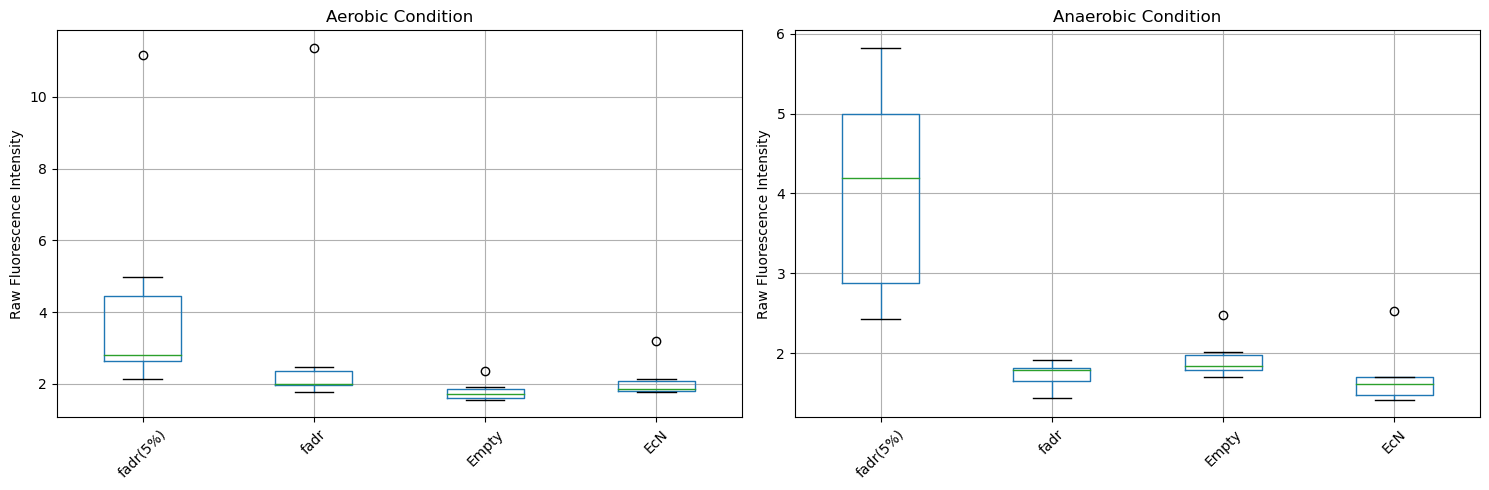
\includegraphics[width=0.8\linewidth]{figures/rawCondition5.png}
	\caption{5\% oleic acid raw fluorescence intensity data box plots}
	\label{fig:5 oleic acid raw data box plots}
\end{figure}

\begin{figure}[h]
	\centering
	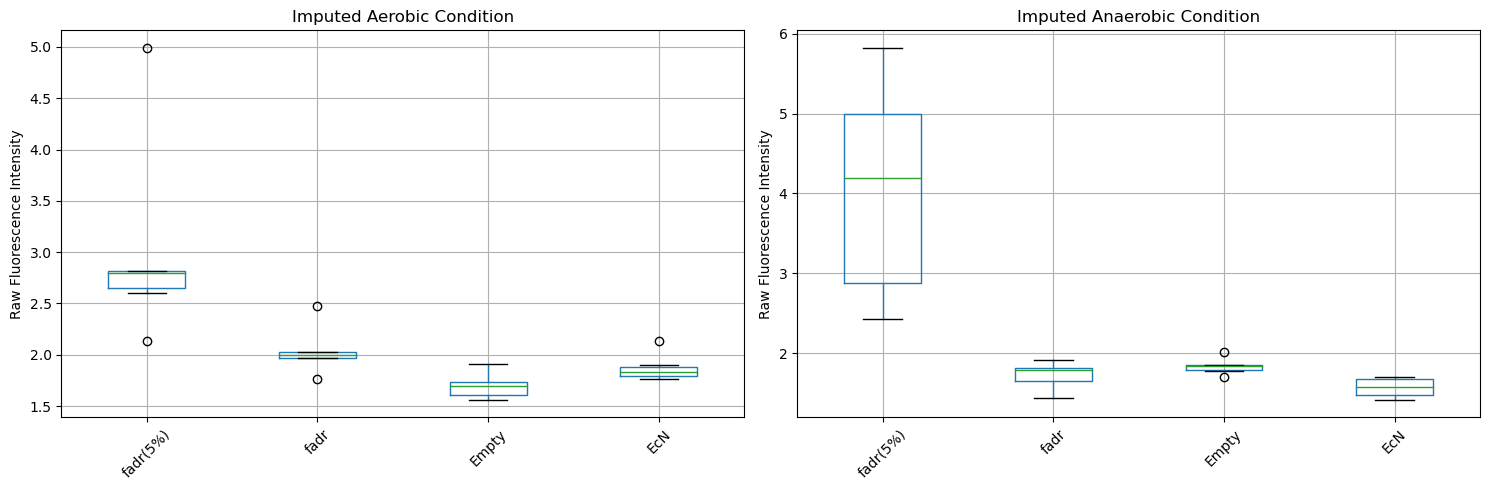
\includegraphics[width=0.8\linewidth]{figures/imputedCondition5.png}
	\caption{5\% oleic acid imputed fluorescence intensity data box plots}
	\label{fig:5 oleic acid imputed data box plots}
\end{figure}


Similarily, for the data of 5\% concentration of oleic acid. The potential outliers in the aerobic data have been imputed using the median values of their respective groups. The raw data box plot and imputed data box plot can be found in Figure \ref{fig:1015 oleic acid imputed data box plots} and Figure \ref{fig:1015 oleic acid imputed data box plots} respectively.

\begin{figure}[h]
	\centering
	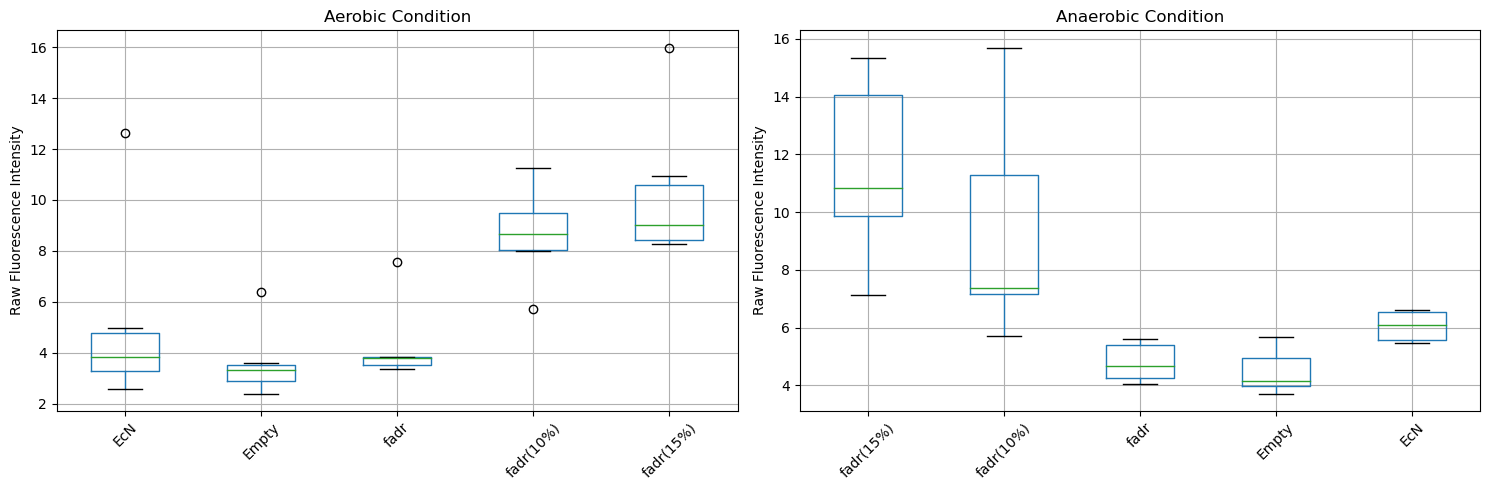
\includegraphics[width=0.8\linewidth]{figures/rawCondition1015.png}
	\caption{10 and 15\% oleic acid raw fluorescence intensity data box plots}
	\label{fig:1015 oleic acid raw data box plots}
\end{figure}

\begin{figure}[h]
	\centering
	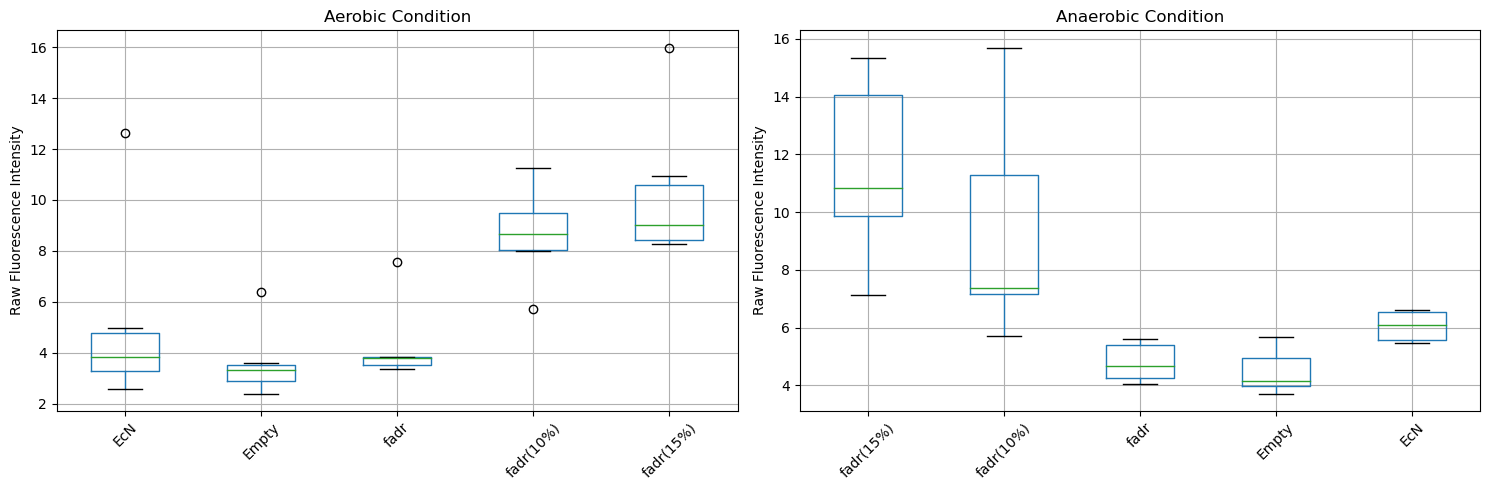
\includegraphics[width=0.8\linewidth]{figures/rawCondition1015.png}
	\caption{10 and 15\% oleic acid imputed fluorescence intensity data box plots}
	\label{fig:1015 oleic acid imputed data box plots}
\end{figure}

\subsection{Calculate the absolute fluorescence intensity}

The correction for background fluorescence is essential to ensure accurate measurements. The sample labeled as fadr serves as a control or baseline and represents the inherent fluorescence that is not due to the specific condition or treatment (in this case, the 5\% condition). By subtracting this background fluorescence, we eliminate any potential interference or noise from non-specific sources. This ensures that the fluorescence intensity we measure for fadr(5\%) is solely due to the 5\% condition, providing a more accurate and representative value.
To calculate the absolute fluorescence intensity from the given data, we need to perform the following operations:

Determination of absolute fluorescence intensity:
For each sample, divide its Raw Fluorescence Intensity by its corresponding OD600 value. This gives the absolute fluorescence intensity(AFI) for that sample.

$$
AFI = \frac{RFI}{OD 600}
$$

Correction for background fluorescence:
To obtain the final fluorescence intensity for the sample labeled as fadr(5\%), subtract the fluorescence intensity of the fadr sample (which acts as a background) from the absolute fluorescence intensity of the fadr(5\%) sample.

$$
	\textbf{Corrected} \quad AFI_{n\%}  = AFI_{n\%} - Empty
$$

Finally, we use the mean corrected absolute fluorescence intensity as the results of experimnets, which are shown below:

$$
\begin{array}{|l|c|c|c|}
	\hline & 5 \% & 10 \% & 15 \% \\
	\hline \text{Aerobic fluorescence intensity}  & 1.9387 & 14.0405 & 16.4747 \\
	\hline \text{Anaerobic fluorescence intensity} & 2.2944 & 12.3819 & 17.6757 \\
	\hline
\end{array}
$$


\end{document}